\documentclass{beamer}
\usefonttheme[onlymath]{serif}
\usepackage{amsmath}
\usepackage{amsfonts}
\usepackage[export]{adjustbox}
\usepackage[utf8]{inputenc}
\usepackage{tikz} 
\usetikzlibrary{bayesnet}

% definitions
\def\H{\mathcal{H}}
\def\X{\mathbf{X}}
\def\w{\mathbf{w}}
\def\W{\mathbf{W}}
\def\const{\mathrm{const}}
\def\Var{\mathrm{Var}}
\def\tr{\mathrm{tr}}
\def\T{\top}
\def\U{\mathbf{U}}
\def\S{\mathbf{S}}
\def\V{\mathbf{V}}
\def\N{\mathcal{N}}
\def\E{\mathbb{E}}
\newcommand{\argmin}{\mathop{\mathrm{argmin}}}
\newcommand{\argmax}{\mathop{\mathrm{argmax}}}
\newcommand{\minimize}{\mathop{\mathrm{minimize}}}
\newcommand{\maximize}{\mathop{\mathrm{maximize}}}
\newcommand{\st}{\mathop{\mathrm{subject\,\,to}}}

%Information to be included in the title page:
\usecolortheme{seahorse}
\title{Infomation Theory}
\author{Thomas Bayes}
\institute{
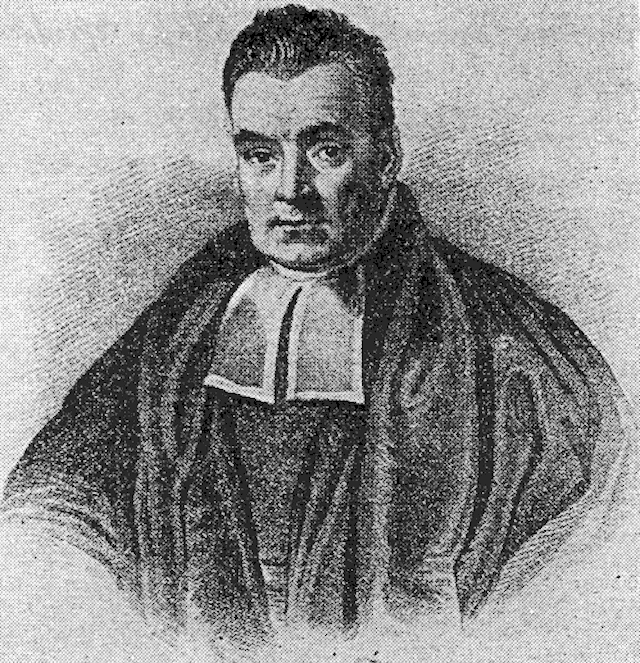
\includegraphics[height=.3\textheight]{../bayes.png}%
}
\date{\today}

    
    
\begin{document}
    
\frame{\titlepage}
\begin{frame}[allowframebreaks]{Introduction}
Lecture Notes for information theory

Reminder for myself of the aim of the note
\begin{itemize}
\item This note should not be a single recording of the lectures. 
\item This note should contain some intuitive understandig of the content covered in the lectures. 
\item Don't try to copy the proof process from the book to this note. Write it on paper, it is a total waste of time and very stupid to write the long proof here. (Writing the main idea of the proof is good)
\item Writing the note firstly make myself review the knowledge, secondly hopefully I can make others who see this note better understand the content in the lectures.
\end{itemize}
## Links
    - [course website](http://www.inference.org.uk/itprnn/book.html)
    - [course materials](http://www.inference.org.uk/itprnn_lectures/)
    ## Lecture 1 : Introduction 
    Various process can be seen as the delivery of the information.
    Information theory is aiming to deliver information even there are noise corrupting the data. We can see the process of the delivering the information as the following steps:
    
    1. the raw data is compressed (encoder)
    2. the compressed data go through a noisy channel
    3. the encoded data is uncompressed (decoder)
    
    The key problem is that how can we make such system more robust to the noise.
    
    > 
    **Example**
    Imaging that we use 0/1 to transfer the information. And the rate of the error is $f$.
    Various ways have been designed such as *parity code*, *repetition code*. Using this code make the probablity of the error lower, however the information delivery rate will be lower.
    We want such a system that with **high delivery rate** and **low loss probablity**.
    Shannon's noisy-channel coding theorem proves that the the error rate can be arbitrarily low when the transfer rate of the information is 
    $$C_{BSC}(f)=1-H_2(f)\\ 
    H_2(f)= f\log_2 \frac{1}{f} + (1-f)\log_2\frac{1}{1-f}$$
    **Magic!**
    
    
    
    ## Lecture 2: 
    
    Information flow can be seen as:
    1. The source information is encoded with more compact representation.
    2. It goes through a noisy channel.
    3. It is decoded to get the raw data.
    If we are able to add more redundancy, we can still decode the original information.
    One interesting example is that in such circumstances, we talk to others by typing texts. 
    
    - The information that we'd like to express is the source.
    - We add redundancy using the language.
    - There are probablity $f$ that the texts are corrupted. 
    - We are still able to recover from it because we add some redudancy, so we are able to decode from the encoded information.
    
    The information content is a good loss function that we can maybe use. **(Like in applications of the robotics, if we want the robotics to explore more, this loss function let the robot choose a solution that give the most information from the candidates) Always being greedy to get the most infomation might not be that good**.
    
    Shannon informaiton content of an outcome of probablity of $P(x=a_i)$ is $h(x=a_i)=\log_2 \frac{1}{P(x=a_i)}$ bits.
    > **Question** 
    $h(x)$ is the compressed file length to which we should aspire. (Don't know what does it mean.)
    
    The average shannon entropy is $$H(x) = \sum_x P(x) \log_2 \frac{1}{P(x)}$$ For example, we are playing the weighing problem. Choosing the probablity distribution with higher information entropy makes us know most about the game.
    
    > **Question**
    But what does it mean that we get new information? How to intuitively understand that the info entropy of probablity distribution {0,1} is smaller than {0.5,0.5}?
    
    ## Lecture 3 : Examples for Source coding theorem
    > **Theorem**
    $N$ outcomes from a source $X$ can be compressed into roughly $NH(X)$ bits.
    
    In the example of bent lottery tickets, there are huge probablity that the lottery tickets has fewer than 100/1000 ones, and nearly no probablity that the winning tickets has more than, say, 200 ones. So we do not need to buy those tickets and we have large probablity to win when we just buy small amount of the lottery tickets. **With high probablity, we can encode the information in shorter length.** Using the *source coding theorem*, we have high probablity to encode $2^{1000}$ information using $1000H_2(X)$ **bits** 
    where $$H_2(X)=0.1\log_2(1/0.1)+0.9\log_2(1/0.9)$$
    
    
    ## Lecture 4 : Proof for Source coding theorem
    > **Recap for the source coding theorem**
    When a source $X$ produces $N$ independent outcomes 
    $$x=x_1x_2\cdots x_N$$
    this string is very likely to be one of the $2^{NH(X)}$ typical outcomes, all of which have probablity $$2^{-NH(X)}$$
    
    We want to design a code to compress the data. The following requirements should be met.
    
    - Can be decoded uniquely. (Should be a prefix code)
    - Expected length should be small, which $L(C,X) = \sum_i p_i l_i$ should be small.
    
    If all character is encoded using the same length, when the length of the code used is $l$, then the number of symbol we can encode is $2^l$. If we use some shorter code, say, $1$ for representing some symbol, we can't use 1xxx to represent other symbols. **Intuitively, if we use some shorter code for some symbol, the cost of them is larger.** And quantitively, it is $2^{-l_i}$. 
    > **Theorem** (Krafts inequality)
    If a code is uniquely decoded, then 
    $$\sum_i 2^{-l_i} \le 1$$
    
    > **Definition** 
    A complete code is one that has 
    $$\sum_i 2^{-l_i} = 1$$
    
    
    
    Now we would like to know how can we design such code that has smallest *expected length*. 
    > **Definition** 
    (I believe that Shannon guess the length of each symbol should be the information entropy bits, so he define this way)
    ideal length: $$l_i^*=\log_2\frac{1}{p_i}=h_i$$
    
    And at the same time, we have one instance of the length of each symbol, we would like to validate that if such coding is the best. We make a transformation first, $$q_i = \frac{2^{-l_i}}{Z}$$ 
    where $Z = \sum_i 2^{-l_i}$, which means that 
    $$l_i=\log_2 \frac{1}{q_i}-\log_2Z\\
    \begin{align}
    L(C,X)=&\sum_ip_i(\log_2 \frac{1}{q_i}-\log_2Z)\\
    =&\sum_ip_i\log_2 \frac{1}{p_i} + \sum_ip_i\log\frac{p_i}{q_i}-\log_2Z
    \end{align}$$
      
    >**Gibbs' inequality**
    $$\sum_i p_i \log \frac{p_i}{q_i} \ge 0$$ iff $p_i = q_i$(probablity distribution are the same), this is KL divergence.
    
    Thus, $$L(C,X) \ge H(X)$$ iff $$l_i=\log_2 \frac{1}{p_i}$$ and it is complete code.
    In real life, $l_i^* = \log_2\frac{1}{p_i}$ is not integer, when we use Huffman coding, $$H(X)\le L \lt H(X) + 1$$ 
    
    ## Lecture 5 : What's wrong with Symbol Code and Arithmetic Coding
    (This lecture seems harder than the previous lectures for me to understand)
    
    **Symbol Code**
    $$H(X) \le L \lt H(X) + 1$$ achieve the equality when $l_i^*=\log\frac{1}{p_i}$
    If we have a binomial probability distribution $$P(x=1) = 0.99, P(x=0) = 0.01$$ The expected length is $L=1$, and the entropy is $H=0.08 bits$
    
    > **Example : Guessing Game**
    We can infer the rest part of a english sentence like 'hel', there are high probablity that a 'l' follows, and the probability distribution changes when we get more letters from the given word. 
    There are three properties of this guessing game:
    1. There are predictive distribution that change with context.
    2. The context dependent predictions change when more data come.
    3. Often, the predictive distribution is **very certain**. (The Huffman coding ensure that **on average** the length is smaller than the $best + 1$, so in total the length may be much larger than the entropy.
    
    We need dynamic coding, there exists a gap between the information entropy $H$ and the Huffman coding expected length $L$ for the **highly determinstic probablity distribution**. 
    
    > **Task**
    Suppose we have a probability distribution that is dynamic, it can give us the probability distribution $$P(x_n = a_i|x_1, \dots, x_{n-1})$$ anytime we want.
    Suppose we want to encode a probability distribution that we do not know, the probability distribution can be more precise as we show more and more information to it. 
    
    **Arithmetic coding**
    The binary code length $l(x_1, x_2, \cdots, x_N) \le \log_2 \frac{1}{P(x_1, x_2, \cdots, x_N)} + 2$
    This shows that the **Arithmetic Coding** is very near optimal, because, as the Kraft inequality and Gibbs inequality shows, the optimal binary code length should be $l(x_1, x_2, \cdots, x_N) \ge \log_2 \frac{1}{P(x_1, x_2, \cdots, x_N)}$ to get the least **expected length**. Otherwise, others will be longer.  
    
    **Think I am still not fully understand the lecture 5**
    
    ## Lecture 6: basic for noisy channel communicating
    If we randomly choose a bit in a code that matches the best compression ratio, then the probability must be 0.5, otherwise we can compress more. 
    If a code is perfectly compressed, then the ratio is 0.5, 0.5. No further compression can be made.
    The arithmetic coding is also useful to generate random numbers,(**why**?)
    Introduce the concept of conditional information. 
    $$H(X|Y) = \sum_i H(X|y_i)p(y_i)\\
    H(X,Y)=\sum_{i,j} p_{ij}\log_2 \frac{1}{p_{ij}}\\
    H(X|Y)\le H(X)\\
    H(X|Y)+H(Y)=H(X,Y)\\
    I(X;Y)=H(X)-H(X|Y)=H(Y)-H(Y|X) $$
    Always write probability distribution if we want to infer something.
    
    ## Lecture 7: Information Measures for noisy Channels
    The channel defines a conditional probability, $Q_{j|i}=P(x=b_j|x=a_i)$
    > **Definiton** : Capacity of a channel
    $$C(Q)=\max_{\mathcal{P}_X}I(X;Y)   \text{ and } \mathcal{P}_X \text{ is called the optimal input distribution}$$
    For example, for a binary symmetric channel with error rate $f$, the optimal input distribution is $(\frac{1}{2}, \frac{1}{2})$, 
    $$\begin{align}I(X;Y)&=H(X)-H(X|Y) \\ &= H(p_1(1-f)+(1-p_1)f) - H(f) \end{align}$$
    the maximum is achieved when $p_1=0.5$ and the capacity $C(Q) = 1 - H(f)$
    Shannon's source coding theorem states that **Reliable communication is possible at rates up to $C$**
    
    **Examples**
    
    - We have a channel that can send a, b, c, d signal, and the result will be a, b, c, d respectively. The optimal input distribution will be $(\frac{1}{4}, \frac{1}{4},\frac{1}{4},\frac{1}{4})$ and the capacity is $2 bits$ which makes sense. 
    - We have a channel whose input is 'a, b, c' and the output is 'M, N', and 'a' will become 'M', 'b' has $\frac{1}{2}$ prob to become 'M', and $\frac{1}{2}$ prob to become 'N', 'c' will become 'N'. If we receive a 'M' output, according the probability theory, there are $\frac{1}{3}$ the input is 'b' and $\frac{2}{3}$ that the input is 'a'. If we assume the probability distribution is $\mathcal{P}_X=(\frac{1}{3},\frac{1}{3},\frac{1}{3})$, then the mutual information is $H(Y) - H(Y|X) = 1 - \frac{1}{3} = \frac{2}{3}$
    ** Guess I quite understand this lecture.**
    
    
    ## Lecture 8 : The Noisy Channel Theorem
    
    $$C\equiv \max_{\mathcal{P}_X} I(X;Y)$$
    
    The distribution $\mathcal{P}_X^*$ that achieves the maximum is called the optimal input distribution.
    
    Shannon's noisy channel coding theorem: **Reliable(virtually error-free) communication is possible at rates up to C**  
    > **Sketch of the proof of the Shannon's Noisy Channel Coding Theorem**
    We have seen the example of the noisy typewriter, we can see that an input corresponds to **only** several output. For binary symmetric code channel, if we use the channel for $N$ times, then this is **similar** to the noisy typewriter, because one input usually corresponds to only a **typical set** of output. If $f$ is small for the BSC, then a 0000 code usually will be 0000 or with code with only one 1. 
    The typical set of the output is $2^{NH(Y)}$, for any particular input sequence, the typical set of output is $2^{NH(Y|X)}$(the result of average). So the non-confusable input can be divided to $2^{NH(Y)-NH(Y|X)}\le2^{NC}$ set. **(I don't quite understand this)**
    
    Let's see the (7,4) Hamming Code. When transmitting such code, we will transmit 4 codes at one time, and the 3 other codes is used for finding the error code. 
    $$H=\begin{bmatrix}
        1  & 1 & 1 & 0 & 1 & 0 & 0 \\
        0  & 1 & 1 & 1 & 0 & 1 & 0 \\
        1  & 0 & 1 & 1 & 0 & 0 & 1
    \end{bmatrix} \\ 
    \text{valid transimission : } Ht = \begin{bmatrix} 0 \\ 0 \\0 \end{bmatrix} \text{mod 2}$$ 
    Using such code, if only one bit flips, we can correct the code.
    
    > **Proof of the proof of the Shannon’s Noisy Channel Coding Theorem**
    We have a transmission signal $t$ (Already with the error detection code), and the linear code matrix $H$ will encode the signal $t$, if no error happened, $Ht=0$, if there are noise, $r = t+n$, then $H(t+n) \neq 0$, from $Hn\neq 0 $, we need to infer the $\tilde{n}$.
    When we construct such a matrix $H_{N\times M}$. The syndrome will be $Hn$, we need to infer $\tilde{n}$ from $Hn$. 
    Probability of error composed of two parts, the first part is that the  noise vector is not contained in the typical set. The second part is that the noise vector $n$ is contained in the bag, but there are other noise vector corresponding to the same syndrome as the $\tilde{n}$.
    The error rate because of the second term is 
    $$\begin{align}P(H) &=\sum_{n\in bag}P(n)1(\exists \tilde{n} \in bag:\tilde{n}\neq n\ H(n-\tilde{n})=\vec0)\\
    &\le \sum_{n\in bag}P(n)\sum_{\tilde{n}\neq n \\ \tilde{n} \in bag}1(H(n-\tilde{n})=\vec0)\end{align}$$
    Then we get average on the $H$(arbitrary matrix, each with
    $$\begin{align}<P>_H &= \sum_H P(H)\sum_{n\in bag}P(n)\sum_{\tilde{n}\neq n \\ \tilde{n} \in bag}1(H(n-\tilde{n})=\vec0)\\
    &=\sum_{n\in bag}P(n)\sum_H P(H)\sum_{\tilde{n}\neq n \\ \tilde{n} \in bag}1(H(n-\tilde{n})=\vec{0})\end{align}
    $$
    For a fixed $n-\tilde{n}$, the probability for $h(n-\tilde{n})=0$ is $\frac{1}{2}$. So $$<P>_H=\sum_{n\in bag}P(n)\sum_{\tilde{n}\neq n \\ \tilde{n} \in bag}(\frac{1}{2})^M \le 2^{NH(f)}(\frac{1}{2})^M$$
    
    So the probablity of error is $$P=P_I + P_{II}=P_I+\frac{1}{2^{M-NH_2(f)}}$$
    The proof doesn't seem to progress well. **Need to be determined later**, ask the youtube author or **see the proof on the book.**
    
    
    ## Lecture 9 & 10: Inference
    Suppose we have some data, and we need to decide the process of generating these data. Generally, we will have some **hypothesis**. If we have a dataset $\{x_1,\dots,{x_n}\}$, then we can have two hypothesis. 
    1. These data come from an exponential probability distribution, the parameter is $\lambda$, $P(X=x)=e^{-\frac{x}{\lambda}}$
    2. These data come from two exponential probability distribution, the parameter are $\lambda_1$ and $\lambda_2$. And we have two decide the data from cluster 1 or cluster 2. 
    >**Hypothesis 1 : Data come from one probability distribution**
    To infer the best parameter, we use Baye's theorem.
    $$P(\lambda|\{x\}, \mathcal{H}_1)=\frac{P(\{x\}|\lambda,\mathcal{H}_1)P(\lambda|\mathcal{H}_1)}{P(\{x_n\}|\mathcal{H}_1)}$$
    **Hypothesis 2 : Data come from two probability distribution**
    In such hypothesis, we need to decide the label for each data point.
    And we can also compare the plausibility of each hypothesis, to decide which model is more plausible $P(\{x_n\}|\mathcal{H}_1)$ and $P(\{x_n\}|\mathcal{H}_2)$
    
    ## Lecture 11 : Clustering as an inference problem
    introduce the K-means algorithm, normal K-means and soft K-means.
    Here we only introduce the soft K-means algorithm (version 1 and version 2)
    ### Soft K-means version 1
    Set the relevance for each point to each mean point.
    \begin{equation*}
    r^{( n)}_{k} =\frac{e^{-\beta d\left( m^{( k)} ,x^{( n)}\right)}}{\sum _{k'} e^{-\beta d\left( m^{( k')} ,x^{( n)}\right)}}
    \end{equation*}
    Then update the mean point. 
    
    \begin{equation*}
    m^{( k)} =\frac{\sum ^{N}_{n=1} r^{( n)}_{k} x^{( n)}}{\sum ^{N}_{n=1} r^{( n)}_{k}}
    \end{equation*}
    ### Soft K-means version 2
    The first version's $\beta $ need to be decided manually, we can guess from the data. **We assume that the data come from the axis-aligned gaussian distribution**.
    
    \begin{equation*}
    {\sigma ^{( k)}_{i}}^{2} =\frac{\sum ^{N}_{n=1} r^{( n)}_{k}\left( x^{( n)}_{i} -m^{( k)}_{i}\right)^{2}}{\sum ^{N}_{n=1} r^{( n)}_{k}}
    \end{equation*}
    Through this way we put less constraint to the data and get better results.
    
    ## Lecture 12 : MCMC
    We now have some probability toolbox. 
    1. Complete enumeration
    2. Laplace's method *See this chapter in the book*
    3. Monte Carlo methods
    4. Variational methods
    
    ### Monte Carlo methods
    We have a posterior probability distribution:
    
    \begin{equation*}
    P( \theta |\{x\}) =\frac{P(\{x\} |\theta ) P( \theta )}{P(\{x\})}
    \end{equation*}
    $P(\{x\})$ are hard the evaluate, $P(\{x\} |\theta ) P( \theta )$ are easy to evaluate. And we want to get the value concerning the $P( \theta |\{x\})$. 
    
    \begin{equation*}
    P( \theta ) =\frac{P^{*}( \theta )}{Z}
    \end{equation*}
    We want to get some data from the probability distritbution $x^{( r)} \sim P$, and we may want to evaluate the value $\Phi ( x) \equiv \int \phi ( x) P( x)$.
    ### Importance Sampling
    We can set a sampler function that we can sample from $Q( x)$. We can evaluate the 
    \begin{equation*}
    \hat{\Phi } =\frac{\sum ^{R}_{r=1}\frac{P^{*}\left( x^{( r)}\right)}{Q\left( x^{( r)}\right) Z} \phi \left( x^{( r)}\right)}{\sum ^{R}_{r=1}\frac{P^{*}\left( x^{( r)}\right)}{Q\left( x^{( r)}\right) Z}} \ 
    \end{equation*}
    We can see that the expectation of $\hat{\Phi }$ if we sample from $Q( x)$ sufficient times is (if $Z$ is not dependent on the value of $x$
    \begin{equation*}
    \int \frac{P^{*}( x)}{Q( x) Z} Q( x) \phi ( x) dx=\int P( x) \phi ( x) dx
    \end{equation*}
    
    which is what we want.
    ### Rejection Sampling
    Another method I do not really know why it does the sampling this way.
    Find $c$ and $Q( x)$ that satisfies $\forall x\ cQ( x) \geqslant P^{*}( x)$, and do sampling in the following steps. 
    1. $x\sim Q( x)$
    2. $u\sim \text{Uniform(} 0,cQ( x)\text{)}$
    3. if $u< P^{*}( x)$ then ACCEPT, else reject. 
    **Question: How to evaluate the $\int P( x) \phi ( x) dx$? See book**
    
    ### Metropolis method
    New way of defining the function $Q( x)$, define it to be $Q( x;x')$ where $x$ is the next location, and $x'$ is the current location. 
    Here is how metropolis method work. 
    1. generate $x\sim Q\left( x;x^{( t)}\right)$
    2. compute acceptance ratio **(why define this way)**
    \begin{equation*}
    a=\frac{P^{*}( x) Q\left( x^{( t)} ;x\right)}{P^{*}\left( x^{( t)}\right) Q\left( x;x^{( t)}\right)}
    \end{equation*}
    3. if $a >1$, accept. Otherwise accept $x$ with probability $a$, accept: $x^{( t+1)} =x$, reject: $x^{( t+1)} =x^{( t)}$
    
    ### Gibbs sampling
    Let's consider a binary probability distribution. $P( x_{1} ,\ x_{2})$
    Assume that we can sample for conditional distribution, $P( x_{1} |x_{2}) ,\ P( x_{2} |x_{1})$. K-means is maybe in such case. It is hard to estimate the probability of $P( x_{1} ,x_{2})$. 
    The following two steps is carried out iteratively. 
    
    \begin{gather*}
    x^{t+1} \sim P\left( x_{1} |x^{t}_{2}\right)\\
    x^{t+1}_{2} \sim P\left( x_{2} |x^{t}_{1}\right)
    \end{gather*}
    In the case of K-means, $x_{1}$ is the parameter of gaussian distribution. $x_{2}$ is the assignment of the data points. **Not so sure** If we cumulate the $P\left( x_{1} |x^{t}_{2}\right)$, then we are able to get the approximate marginal distribution of $P( x_{1})$.
    
    
    ## Lecture 13
    The three methods above have problems. 1. Random walk behavior (don't know what's wrong with it) 2. Sensitivity to step size. 3. Don't know when to stop. 
    Slice sampling and exact sampling are more efficient sample method. 
    Hamilton methods, the key is to add the momentum to the energy.
    Overrelaxation can be added to the Gibb's sampling. The key is that you do not sample from the original conditional distribution but you sample in some biased conditional distribution. Can be applied when all the conditional distribution are gaussians.
    ### Ordered Gibbs sampling 
    get K samples from the conditional distribution, and plus the start point, and **go to the other end of the point**
    The methods above, solve the problem of random walk behavior. 
    The methods below will get down to solve 
    
    Gibbs sampling can work if we can get samples from the conditional probability distribution.
    
    ### Slice Sampling
    a method, for detail, **see books**
    
    ## Lecture 14 : Variational Method
    All previous method all deal with the nasty probability distribution. 
    Laplace's method deals with the nasty probability distribution by approximating the probability distribution with the gaussian distribution.
    The main idea of the variational method is that we can approximate the probability distribution by some probability distribution we know with some parameters, then we save some objective function such as KL divergence to get the optimal parameters. 
    ** See the content of the variational method and see the rest of the video lectures (starting from the problem of the spin system** 
    See it carefully, 
    
    ## Notes about Bayesian inference
    
    
    

\end{frame}


\end{document}